\documentclass{standalone}
\usepackage{standalone}

\begin{document}
\section{Mapping Using Naive BWT FM-index}
BWT FM-index \cite{fm_index} is implemented naively at first.  The main idea is if a long chunk of a read could be mapped to a long chunk of the reference, then the probability of this mapping to be accurate is quite high. One of the main drawback of NanoBLASTer \cite{nanoBLAST} is it could not detect a long insertion or a long deletion. In this approach, the main goal is approaching this type of problem.

If two long chunks of a read is mapped to very close distance in reference but long distance in read, then it indicates that there is a long insertion in the read. Similarly, if these two mapped chunks maintain a long distance between them in reference but very short distance in read then there exists a long deletion in the read. Figure \ref{fig:longMapDeleltion} and \ref{fig:longMapInsertion} make the idea more clear. The red portions indicate the long k-mers and the arrows indicates from read where they are mapped in reference.

\begin{figure}
	\centering

	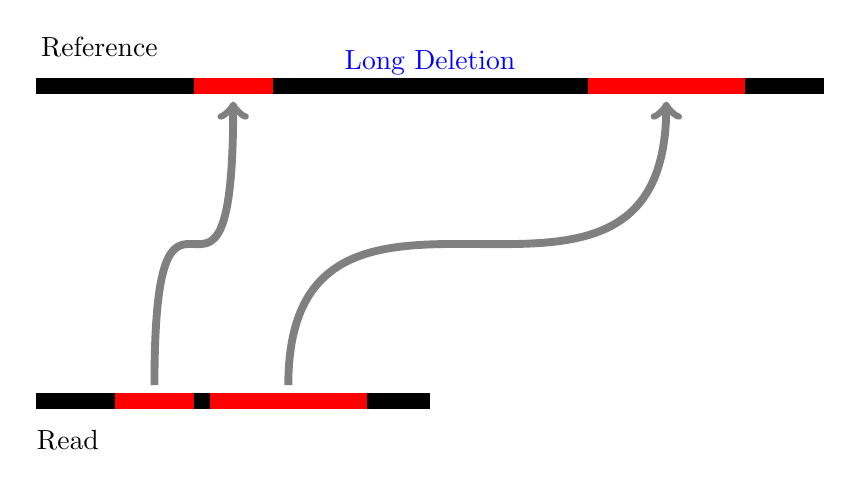
\begin{tikzpicture}[]
	
	%reference
	\draw[line width=2mm] (0,4) -- (10,4);
	\draw[line width=2mm,color=red] (2,4) -- (3,4);
	\draw[line width=2mm,color=red] (7,4) -- (9,4);
	%read
	\draw[line width=2mm] (0,0) -- (5,0);
	\draw[line width=2mm,color=red] (1,0) -- (2,0);
	\draw[line width=2mm,color=red] (2.2,0) -- (4.2,0);
	%labels
	\node[rectangle](refer) at (0.8,4.5) {Reference};
	\node[rectangle,color=blue](refer) at (5,4.3) {Long Deletion};
	\node[rectangle](refer) at (0.4,-0.5) {Read};
	%arrows
	\draw[line width=1mm,color=black!50,->] (1.5,0.2) ..  controls (1.5,3.8) and (2.5,0.2) .. (2.5,3.8);
	\draw[line width=1mm,color=black!50,->] (3.2,0.2) .. controls(3.2,3.8) and (8,0.2) .. (8,3.8);
	\end{tikzpicture}
	\caption{Mapping Two Long K-mers with Long Deletion in Read.} \label{fig:longMapDeleltion}
\end{figure}
\begin{figure}
	\centering
	
	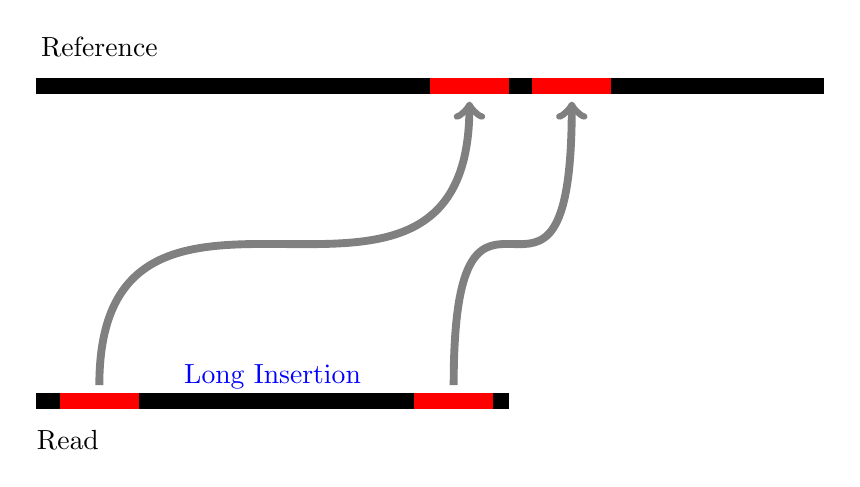
\begin{tikzpicture}[]
	%reference
	\draw[line width=2mm] (0,4) -- (10,4);
	\draw[line width=2mm,color=red] (5,4) -- (6,4);
	\draw[line width=2mm,color=red] (6.3,4) -- (7.3,4);
	%reads
	\draw[line width=2mm] (0,0) -- (6,0);
	\draw[line width=2mm,color=red] (0.3,0) -- (1.3,0);
	\draw[line width=2mm,color=red] (4.8,0) -- (5.8,0);
	%labels
	\node[rectangle](refer) at (0.8,4.5) {Reference};
	\node[rectangle,color=blue](refer) at (3,0.3) {Long Insertion};
	\node[rectangle](refer) at (0.4,-0.5) {Read};
	%arrows
	\draw[line width=1mm,color=black!50,->] (0.8,0.2) ..  controls (0.8,3.8) and (5.5,0.2) .. (5.5,3.8);
	\draw[line width=1mm,color=black!50,->] (5.3,0.2) .. controls(5.3,3.8) and (6.8,0.2) .. (6.8,3.8);
	\end{tikzpicture}
	\caption{Mapping Two Long K-mer with Long Insertion in Read.} \label{fig:longMapInsertion}
\end{figure}

So, from a certain value of $K$, we would check in the FM-index whether the $K$-mer exists in the reference or not. If we get any null set of location as result, we would consider the last not-null set of locations. That means, for an increasing $K$, if we get no location in the reference for that $K$-mer, then we would stop increasing the value of $K$ and would work with the locations we get for $K-1$. Algorithm \ref{alg:inc_K_FM} may help to understand better. Figure \ref{fig:NaiveFM1} through \ref{fig:NaiveFM6} visualize the implementation.

\begin{algorithm}
	\caption{Mapping K-mers of Variable Lengths of a Read to Reference Using Naive FM-index }
	\label{alg:inc_K_FM}
	\begin{algorithmic}[1]
		\Require $K_{min}$ is the minimum length of K or the starting length of K, $fmIndex$ is the indexed reference which is basically a data structure, $read$ is the particular Read Sequence. 
		\Ensure A list of K-mers with their position in read and reference.
		\Function{MapWithNaiveFM}{$fmIndex, read, minK$}
		\Local{$i, j, readLength, kmer, countOcc, kmer_{prev}, locations, retList$}
		\Let{$readLength$}{|read|} 
		\Comment{|s| means length of the string s}
		\Let{retList}{$null$} 
		\For{$i \leftarrow 0$ \textbf{to} $readLength - K_{min}$}
		\Let{kmer_{prev}}{$null$} 
		\For{$j \leftarrow K_{min}$ \textbf{to} $readLength - i + 1$} 
		\Let{kmer}{$read[ i : i + j ]$}
		\Comment{\parbox[t]{.5\linewidth}}{$s[a:b]$ means substring consisting of characters from index a(inclusive) to index b(exclusive) of string s}
		\Let{countOcc}{$CountFM(fmIndex, kmer)$} \label{alg:inc_K_FM:9}
		\Comment{\parbox[t]{.4\linewidth}}{\emph{CountFM} function takes two parameters, an \emph{FM-index} data structure, a string and returns the count of occurrences of the string in the data structure}
		\If{$countOcc = 0$}
		\textbf{break}
		\EndIf
		\Let{kmer_{prev}}{$kmer$} 
		\EndFor 
		\If{$kmer_{prev}$ \textbf{not \emph{null}}}
		\Let{locations}{LocateFM(fmIndex, kmer_{prev})}
		\Comment{\parbox[t]{.3\linewidth}}{\emph{LocateFM} function takes two parameters, an \emph{FM-index} data structure, a string and returns the locations of occurrences of the string in the data structure}
		\State{\textbf{Append} $(kmer_{prev}, i, locations)$ to $retList$}
		\Let{i}{i + j - 1} 
		\EndIf
		\EndFor
		\State\Return{retList}
		\EndFunction
		
	\end{algorithmic}
	\end{algorithm}
	
	\begin{figure}
		\centering
		\tikzstyle{block} = [rectangle, draw, line width=0.5mm,
		text centered]
		\begin{tikzpicture}[]
		%variables
		\newcommand{\arrowStartX}{5.13}
		\newcommand{\arrowStartY}{1.3}
		\newcommand{\arrowEndY}{3.8}
		%reference
		\draw[line width=2mm] (0,4) -- (10,4);
		%\draw[line width=2mm,color=red] (5,4) -- (6,4);
		%\draw[line width=2mm,color=red] (6.3,4) -- (7.3,4);
		
		%labels
		\node[rectangle](refer) at (0.8,4.5) {Reference};
		\node[rectangle,rotate=-90, ultra thick](refer) at (5.13,0.7) {\fontsize{93}{72.4}\selectfont\{};
		\node[rectangle](refer) at (5.1,-0.5) {K-mer from Read};
		

		%arrows
		\draw[line width=1mm,color=black!50,->] (\arrowStartX,\arrowStartY) -- (0.5,\arrowEndY);
		\draw[line width=2mm,color=red] (0.4,4) -- (0.6,4);
		\draw[line width=1mm,color=black!50,->] (\arrowStartX,\arrowStartY) -- (1.4,\arrowEndY);
		\draw[line width=2mm,color=red] (1.3,4) -- (1.5,4);
		\draw[line width=1mm,color=black!50,->] (\arrowStartX,\arrowStartY) -- (2.4,\arrowEndY);
		\draw[line width=2mm,color=red] (2.3,4) -- (2.5,4);
		\draw[line width=1mm,color=black!50,->] (\arrowStartX,\arrowStartY) -- (3.2,\arrowEndY);
		\draw[line width=2mm,color=red] (3.1,4) -- (3.3,4);
		\draw[line width=1mm,color=black!50,->] (\arrowStartX,\arrowStartY) -- (4.1,\arrowEndY);
		\draw[line width=2mm,color=red] (4,4) -- (4.2,4);
		\draw[line width=1mm,color=black!50,->] (\arrowStartX,\arrowStartY) -- (4.9,\arrowEndY);
		\draw[line width=2mm,color=red] (4.8,4) -- (5,4);
		\draw[line width=1mm,color=black!50,->] (\arrowStartX,\arrowStartY) -- (5.7,\arrowEndY);
		\draw[line width=2mm,color=red] (5.6,4) -- (5.8,4);
		\draw[line width=1mm,color=black!50,->] (\arrowStartX,\arrowStartY) -- (6.9,\arrowEndY);
		\draw[line width=2mm,color=red] (6.8,4) -- (7,4);
		\draw[line width=1mm,color=black!50,->] (\arrowStartX,\arrowStartY) -- (7.4,\arrowEndY);
		\draw[line width=2mm,color=red] (7.3,4) -- (7.5,4);
		\draw[line width=1mm,color=black!50,->] (\arrowStartX,\arrowStartY) -- (8.2,\arrowEndY);
		\draw[line width=2mm,color=red] (8.1,4) -- (8.3,4);
		\draw[line width=1mm,color=black!50,->] (\arrowStartX,\arrowStartY) -- (9,\arrowEndY);
		\draw[line width=2mm,color=red] (8.9,4) -- (9.1,4);
		\draw[line width=1mm,color=black!50,->] (\arrowStartX,\arrowStartY) -- (9.7,\arrowEndY);
		\draw[line width=2mm,color=red] (9.6,4) -- (9.8,4);
		%read
		\node [block] (Val1_1) at (4,0) {A};
		\node [block, anchor=west] (Val1_2) at (Val1_1.east) {T};
		\node [block, anchor=west] (Val1_3) at (Val1_2.east) {T};
		\node [block, anchor=west] (Val1_4) at (Val1_3.east) {C};
		\node [block, anchor=west] (Val1_5) at (Val1_4.east) {G};

		\end{tikzpicture}
		\caption{A K-mer with Value $K = K_{min}$ is Picked Up from Read and Indicated Where The K-mer is Found in the Reference.} \label{fig:NaiveFM1}
	\end{figure}
	\begin{figure}
		\centering
		\tikzstyle{block} = [rectangle, draw, line width=0.5mm,
		text centered]
		\begin{tikzpicture}[]
		%variables
		\newcommand{\arrowStartX}{5.15}
		\newcommand{\arrowStartY}{1.4}
		\newcommand{\arrowEndY}{3.8}
		%reference
		\draw[line width=2mm] (0,4) -- (10,4);
		%\draw[line width=2mm,color=red] (5,4) -- (6,4);
		%\draw[line width=2mm,color=red] (6.3,4) -- (7.3,4);
		
		%labels
		\node[rectangle](refer) at (0.8,4.5) {Reference};
		\node[rectangle,rotate=-90, ultra thick](refer) at (5.17,0.8) {\fontsize{112}{72.4}\selectfont\{};
		\node[rectangle](refer) at (5.1,-0.5) {$(K+1)$-mer from Read};
		
		
		%arrows
		
		\draw[line width=1mm,color=black!50,->] (\arrowStartX,\arrowStartY) -- (1.4,\arrowEndY);
		\draw[line width=2mm,color=red] (1.3,4) -- (1.5,4);
		
		\draw[line width=1mm,color=black!50,->] (\arrowStartX,\arrowStartY) -- (2.4,\arrowEndY);
		\draw[line width=2mm,color=red] (2.3,4) -- (2.5,4);
		
		\draw[line width=1mm,color=black!50,->] (\arrowStartX,\arrowStartY) -- (3.2,\arrowEndY);
		\draw[line width=2mm,color=red] (3.1,4) -- (3.3,4);
		
		\draw[line width=1mm,color=black!50,->] (\arrowStartX,\arrowStartY) -- (4.9,\arrowEndY);
		\draw[line width=2mm,color=red] (4.8,4) -- (5,4);
		
		\draw[line width=1mm,color=black!50,->] (\arrowStartX,\arrowStartY) -- (6.9,\arrowEndY);
		\draw[line width=2mm,color=red] (6.8,4) -- (7,4);
		
		\draw[line width=1mm,color=black!50,->] (\arrowStartX,\arrowStartY) -- (8.2,\arrowEndY);
		\draw[line width=2mm,color=red] (8.1,4) -- (8.3,4);
		
		\draw[line width=1mm,color=black!50,->] (\arrowStartX,\arrowStartY) -- (9,\arrowEndY);
		\draw[line width=2mm,color=red] (8.9,4) -- (9.1,4);
		
		\draw[line width=1mm,color=black!50,->] (\arrowStartX,\arrowStartY) -- (9.7,\arrowEndY);
		\draw[line width=2mm,color=red] (9.6,4) -- (9.8,4);
		
		%read
		\node [block] (Val1_1) at (3.75,0) {A};
		\node [block, anchor=west] (Val1_2) at (Val1_1.east) {T};
		\node [block, anchor=west] (Val1_3) at (Val1_2.east) {T};
		\node [block, anchor=west] (Val1_4) at (Val1_3.east) {C};
		\node [block, anchor=west] (Val1_5) at (Val1_4.east) {G};
		\node [block, anchor=west] (Val1_6) at (Val1_5.east) {C};
		\end{tikzpicture}
		\caption{Extending One Base in $K$-mer From Read in Figure \ref{fig:NaiveFM1}, $(K+1)$-mer is Found. The Locations of This $(K+1)$-mer in the Reference is Reduced. } \label{fig:NaiveFM2}
	\end{figure}
	\begin{figure}
		\centering
		\tikzstyle{block} = [rectangle, draw, line width=0.5mm,
		text centered]
		\begin{tikzpicture}[]
		%variables
		\newcommand{\arrowStartX}{5.46}
		\newcommand{\arrowStartY}{1.5}
		\newcommand{\arrowEndY}{3.8}
		%reference
		\draw[line width=2mm] (0,4) -- (10,4);
		%\draw[line width=2mm,color=red] (5,4) -- (6,4);
		%\draw[line width=2mm,color=red] (6.3,4) -- (7.3,4);
		
		%labels
		\node[rectangle](refer) at (0.8,4.5) {Reference};
		\node[rectangle,rotate=-90, ultra thick](refer) at (5.46,0.85) {\fontsize{130}{72.4}\selectfont\{};
		\node[rectangle](refer) at (5.3,-0.5) {$(K+2)$-mer from Read};
		
		
		%arrows
		
		\draw[line width=1mm,color=black!50,->] (\arrowStartX,\arrowStartY) -- (1.4,\arrowEndY);
		\draw[line width=2mm,color=red] (1.2,4) -- (1.5,4);
		
		\draw[line width=1mm,color=black!50,->] (\arrowStartX,\arrowStartY) -- (8.2,\arrowEndY);
		\draw[line width=2mm,color=red] (8,4) -- (8.3,4);
		

		
		\draw[line width=1mm,color=black!50,->] (\arrowStartX,\arrowStartY) -- (9.7,\arrowEndY);
		\draw[line width=2mm,color=red] (9.5,4) -- (9.8,4);
		
		%read
		\node [block] (Val1_1) at (3.75,0) {A};
		\node [block, anchor=west] (Val1_2) at (Val1_1.east) {T};
		\node [block, anchor=west] (Val1_3) at (Val1_2.east) {T};
		\node [block, anchor=west] (Val1_4) at (Val1_3.east) {C};
		\node [block, anchor=west] (Val1_5) at (Val1_4.east) {G};
		\node [block, anchor=west] (Val1_6) at (Val1_5.east) {C};
		\node [block, anchor=west] (Val1_7) at (Val1_6.east) {A};
		\end{tikzpicture}
		\caption{Extending One More Base From Figure \ref{fig:NaiveFM2}, $(K+2)$-mer is Constructed. The Locations of This $(K+2)$-mer in the Reference is Reduced And Now It is Only 3. } \label{fig:NaiveFM3}
	\end{figure}
	\begin{figure}
		\centering
		\tikzstyle{block} = [rectangle, draw, line width=0.5mm,
		text centered]
		\begin{tikzpicture}[]
		%variables
		\newcommand{\arrowStartX}{5}
		\newcommand{\arrowStartY}{1.65}
		\newcommand{\arrowEndY}{3.8}
		%reference
		\draw[line width=2mm] (0,4) -- (10,4);
		%\draw[line width=2mm,color=red] (5,4) -- (6,4);
		%\draw[line width=2mm,color=red] (6.3,4) -- (7.3,4);
		
		%labels
		\node[rectangle](refer) at (0.8,4.5) {Reference};
		\node[rectangle,rotate=-90, ultra thick](refer) at (5,0.9) {\fontsize{150}{72.4}\selectfont\{};
		\node[rectangle](refer) at (4.9,-0.5) {$(K+3)$-mer from Read};
		
		
		%arrows
		
		\draw[line width=1mm,color=black!50,->] (\arrowStartX,\arrowStartY) -- (1.4,\arrowEndY);
		\draw[line width=2mm,color=red] (1.1,4) -- (1.7,4);
		
		
		%read
		\node [block] (Val1_1) at (3,0) {A};
		\node [block, anchor=west] (Val1_2) at (Val1_1.east) {T};
		\node [block, anchor=west] (Val1_3) at (Val1_2.east) {T};
		\node [block, anchor=west] (Val1_4) at (Val1_3.east) {C};
		\node [block, anchor=west] (Val1_5) at (Val1_4.east) {G};
		\node [block, anchor=west] (Val1_6) at (Val1_5.east) {C};
		\node [block, anchor=west] (Val1_7) at (Val1_6.east) {A};
		\node [block, anchor=west] (Val1_8) at (Val1_7.east) {A};
		\end{tikzpicture}
		\caption{Continuing the Extension, From Figure \ref{fig:NaiveFM3} $(K+3)$-mer is Created. The Count in Reference is Only One. } \label{fig:NaiveFM4}
	\end{figure}
	\begin{figure}
		\centering
		\tikzstyle{block} = [rectangle, draw, line width=0.5mm,
		text centered]
		\begin{tikzpicture}[]
		%variables
		\newcommand{\arrowStartX}{5.3}
		\newcommand{\arrowStartY}{1.8}
		\newcommand{\arrowEndY}{3.8}
		%reference
		\draw[line width=2mm] (0,4) -- (10,4);
		%\draw[line width=2mm,color=red] (5,4) -- (6,4);
		%\draw[line width=2mm,color=red] (6.3,4) -- (7.3,4);
		
		%labels
		\node[rectangle](refer) at (0.8,4.5) {Reference};
		\node[rectangle,rotate=-90, ultra thick](refer) at (5.27,1.05) {\fontsize{170}{72.4}\selectfont\{};
		\node[rectangle](refer) at (5.15,-0.5) {$(K+4)$-mer from Read};
		
		
		%arrows
		
		\draw[line width=1mm,color=black!50,->] (\arrowStartX,\arrowStartY) -- (1.4,\arrowEndY);
		\draw[line width=2mm,color=red] (1.1,4) -- (1.7,4);
		
		
		%read
		\node [block] (Val1_1) at (3,0) {A};
		\node [block, anchor=west] (Val1_2) at (Val1_1.east) {T};
		\node [block, anchor=west] (Val1_3) at (Val1_2.east) {T};
		\node [block, anchor=west] (Val1_4) at (Val1_3.east) {C};
		\node [block, anchor=west] (Val1_5) at (Val1_4.east) {G};
		\node [block, anchor=west] (Val1_6) at (Val1_5.east) {C};
		\node [block, anchor=west] (Val1_7) at (Val1_6.east) {A};
		\node [block, anchor=west] (Val1_8) at (Val1_7.east) {A};
		\node [block, anchor=west] (Val1_9) at (Val1_8.east) {G};
		\end{tikzpicture}
		\caption{ From Figure \ref{fig:NaiveFM4}, $(K+4)$-mer is Made By Appending One Base From Read. It has No Consequence in The Count in Reference. } \label{fig:NaiveFM5}
	\end{figure}
	\begin{figure}
		\centering
		\tikzstyle{block} = [rectangle, draw, line width=0.5mm,
		text centered]
		\begin{tikzpicture}[]
		%variables
		\newcommand{\arrowStartX}{5}
		\newcommand{\arrowStartY}{1.65}
		\newcommand{\arrowEndY}{3.8}
		%reference
		\draw[line width=2mm] (0,4) -- (10,4);
		%\draw[line width=2mm,color=red] (5,4) -- (6,4);
		%\draw[line width=2mm,color=red] (6.3,4) -- (7.3,4);
		
		%labels
		\node[rectangle](refer) at (0.8,4.5) {Reference};
		\node[rectangle,rotate=-90, ultra thick](refer) at (5.35,1.1) {\fontsize{187}{72.4}\selectfont\{};
		\node[rectangle](refer) at (5.2,-0.5) {$(K+5)$-mer from Read};
		
		
		
		%read
		\node [block] (Val1_1) at (2.8,0) {A};
		\node [block, anchor=west] (Val1_2) at (Val1_1.east) {T};
		\node [block, anchor=west] (Val1_3) at (Val1_2.east) {T};
		\node [block, anchor=west] (Val1_4) at (Val1_3.east) {C};
		\node [block, anchor=west] (Val1_5) at (Val1_4.east) {G};
		\node [block, anchor=west] (Val1_6) at (Val1_5.east) {C};
		\node [block, anchor=west] (Val1_7) at (Val1_6.east) {A};
		\node [block, anchor=west] (Val1_8) at (Val1_7.east) {A};
		\node [block, anchor=west] (Val1_9) at (Val1_8.east) {G};
		\node [block, anchor=west] (Val1_10) at (Val1_9.east) {C};
		\end{tikzpicture}
		\caption{ One Base Extension in $(K+4)$-mer of Figure \ref{fig:NaiveFM5} Generates $(K+5)$-mer. It Shows There is No Existence of Such $(K+5)$-mer in Reference. So, the Locations Got From Figure \ref{fig:NaiveFM5} Would be Considered as Final.} \label{fig:NaiveFM6}
	\end{figure}
\end{document}